\documentclass[12pt,a4paper]{article}

% ============== PACKAGES ==============
\usepackage[margin=1in]{geometry}
\usepackage{graphicx}
\usepackage{tikz}
\usetikzlibrary{automata, positioning, arrows.meta, shapes.geometric}
\usepackage{xcolor}
\usepackage{listings}
\usepackage{tcolorbox}
\tcbuselibrary{skins}
\usepackage{fancyhdr}
\usepackage{titlesec}
\usepackage{amsmath}
\usepackage{booktabs}
\usepackage{enumitem}
\usepackage{hyperref}

% ============== SOLARIZED LIGHT COLORS ==============
\definecolor{solarizedBase03}{HTML}{002B36}
\definecolor{solarizedBase02}{HTML}{073642}
\definecolor{solarizedBase01}{HTML}{586E75}
\definecolor{solarizedBase00}{HTML}{657B83}
\definecolor{solarizedBase0}{HTML}{839496}
\definecolor{solarizedBase1}{HTML}{93A1A1}
\definecolor{solarizedBase2}{HTML}{EEE8D5}
\definecolor{solarizedBase3}{HTML}{FDF6E3}
\definecolor{solarizedYellow}{HTML}{B58900}
\definecolor{solarizedOrange}{HTML}{CB4B16}
\definecolor{solarizedRed}{HTML}{DC322F}
\definecolor{solarizedMagenta}{HTML}{D33682}
\definecolor{solarizedViolet}{HTML}{6C71C4}
\definecolor{solarizedBlue}{HTML}{268BD2}
\definecolor{solarizedCyan}{HTML}{2AA198}
\definecolor{solarizedGreen}{HTML}{859900}

% Mac-style colors
\definecolor{macRed}{HTML}{FF5F56}
\definecolor{macYellow}{HTML}{FFBD2E}
\definecolor{macGreen}{HTML}{27C93F}

% ============== LISTINGS SETUP ==============
\lstdefinestyle{vhdlstyle}{
    language=VHDL,
    basicstyle=\ttfamily\small\color{solarizedBase00},
    keywordstyle=\color{solarizedBlue}\bfseries,
    commentstyle=\color{solarizedBase1}\itshape,
    stringstyle=\color{solarizedCyan},
    numberstyle=\tiny\color{solarizedBase1},
    numbers=left,
    numbersep=8pt,
    breaklines=true,
    showstringspaces=false,
    tabsize=3,
    backgroundcolor=\color{solarizedBase3},
    frame=single,
    rulecolor=\color{solarizedBase2},
    morekeywords={library, use, entity, port, is, end, architecture, begin,
                  process, if, then, else, elsif, case, when, signal, type,
                  downto, others, rising_edge, std_logic, std_logic_vector,
                  in, out, and, or, not, xor, nand, nor},
    literate={<=}{{\textcolor{solarizedOrange}{<=}}}2
             {=>}{{\textcolor{solarizedOrange}{=>}}}2
             {:=}{{\textcolor{solarizedOrange}{:=}}}2,
}

% Mac-style code header
\newcommand{\macheader}[1]{%
\vspace{0.3cm}
\noindent
\begin{tikzpicture}
    \node[
        fill=solarizedBase2,
        rounded corners=6pt,
        minimum width=\linewidth-0.5pt,
        minimum height=0.7cm,
        anchor=north west
    ] (header) {};
    \fill[macRed] ([xshift=12pt]header.west) circle (5pt);
    \fill[macYellow] ([xshift=26pt]header.west) circle (5pt);
    \fill[macGreen] ([xshift=40pt]header.west) circle (5pt);
    \node[anchor=east, font=\ttfamily\small\color{solarizedBase01}] at ([xshift=-10pt]header.east) {#1};
\end{tikzpicture}
\vspace{-0.35cm}
}

% ============== HEADER/FOOTER ==============
\pagestyle{fancy}
\fancyhf{}
\fancyhead[L]{\small DSD Lab 04}
\fancyhead[R]{\small FA23-BCE-113}
\fancyfoot[C]{\thepage}
\renewcommand{\headrulewidth}{0.4pt}

% ============== TITLE FORMATTING ==============
\titleformat{\section}{\Large\bfseries\color{solarizedBlue}}{\thesection}{1em}{}
\titleformat{\subsection}{\large\bfseries\color{solarizedCyan}}{\thesubsection}{1em}{}

% ============== DOCUMENT ==============
\begin{document}

% ============== TITLE PAGE ==============
\begin{titlepage}
    \centering
    \vspace*{1cm}
    {\Huge\bfseries Lab \# 04\par}
    \vspace{0.5cm}
    {\LARGE Finite State Machines using VHDL\par}
    \vspace{1cm}
    {\Large\itshape Digital System Design\par}
    \vspace{2cm}

    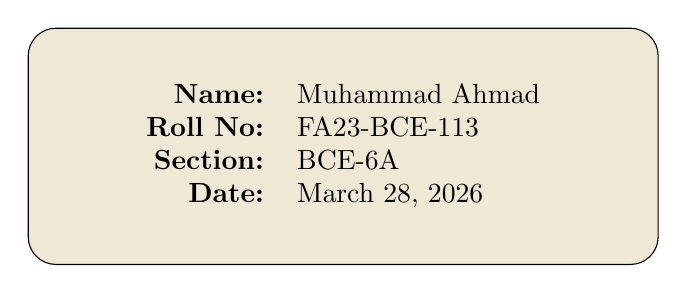
\begin{tikzpicture}
        \node[draw, rounded corners=10pt, fill=solarizedBase2, minimum width=8cm, minimum height=3cm] {
            \begin{tabular}{rl}
                \textbf{Name:} & Muhammad Ahmad \\
                \textbf{Roll No:} & FA23-BCE-113 \\
                \textbf{Section:} & BCE-6A \\
                \textbf{Date:} & March 28, 2026
            \end{tabular}
        };
    \end{tikzpicture}

    \vfill
    {\large Department of Computer Engineering\\
    HITEC University, Taxila\par}
\end{titlepage}

% ============== TABLE OF CONTENTS ==============
\tableofcontents
\newpage

% ============== MOORE VS MEALY DISCUSSION ==============
\section{Moore vs Mealy Machines: A Comparative Analysis}

\subsection{Moore Machine}
\begin{itemize}[leftmargin=*]
    \item \textbf{Output depends ONLY on current state}
    \item Output changes synchronously with state transitions
    \item Generally requires more states than Mealy
    \item Output is more stable (no glitches from input changes)
    \item Easier to design and debug
\end{itemize}

\begin{center}
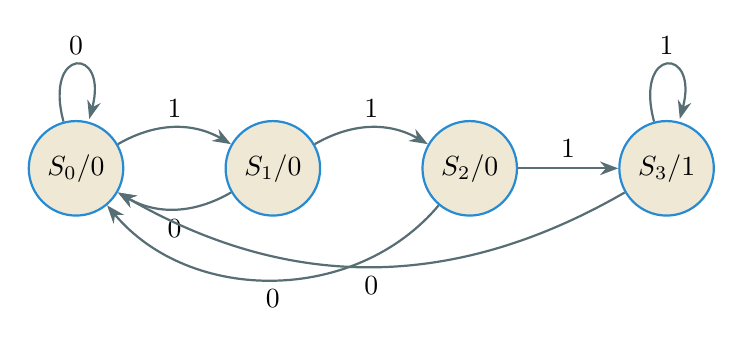
\begin{tikzpicture}[
    ->,>=Stealth,
    node distance=2.5cm,
    every state/.style={draw=solarizedBlue, fill=solarizedBase2, thick, minimum size=1.2cm},
    every edge/.style={draw=solarizedBase01, thick}
]
    \node[state] (S0) {$S_0/0$};
    \node[state, right of=S0] (S1) {$S_1/0$};
    \node[state, right of=S1] (S2) {$S_2/0$};
    \node[state, right of=S2] (S3) {$S_3/1$};

    \path (S0) edge[loop above] node{0} (S0)
          (S0) edge[bend left] node[above]{1} (S1)
          (S1) edge[bend left] node[below]{0} (S0)
          (S1) edge[bend left] node[above]{1} (S2)
          (S2) edge[bend left=50] node[below]{0} (S0)
          (S2) edge node[above]{1} (S3)
          (S3) edge[bend left] node[below]{0} (S0)
          (S3) edge[loop above] node{1} (S3);
\end{tikzpicture}
\end{center}
\begin{center}
    \textit{Figure 1: Moore Machine for "111" Detection (Output delayed by one cycle)}
\end{center}

\subsection{Mealy Machine}
\begin{itemize}[leftmargin=*]
    \item \textbf{Output depends on current state AND current input}
    \item Output changes immediately when input changes (asynchronous)
    \item Generally requires fewer states than Moore
    \item Faster response (output appears same cycle as input)
    \item More prone to glitches if input is noisy
\end{itemize}

\begin{center}
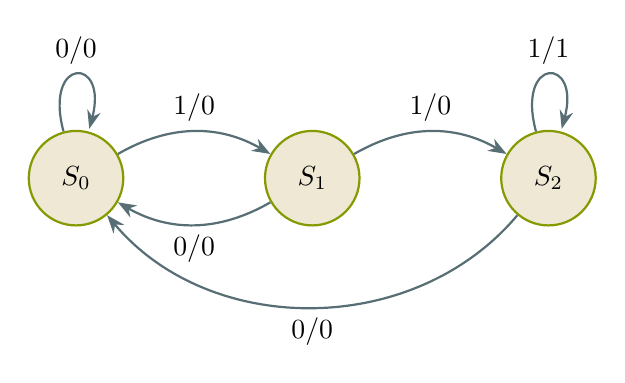
\begin{tikzpicture}[
    ->,>=Stealth,
    node distance=3cm,
    every state/.style={draw=solarizedGreen, fill=solarizedBase2, thick, minimum size=1.2cm},
    every edge/.style={draw=solarizedBase01, thick}
]
    \node[state] (S0) {$S_0$};
    \node[state, right of=S0] (S1) {$S_1$};
    \node[state, right of=S1] (S2) {$S_2$};

    \path (S0) edge[loop above] node{0/0} (S0)
          (S0) edge[bend left] node[above]{1/0} (S1)
          (S1) edge[bend left] node[below]{0/0} (S0)
          (S1) edge[bend left] node[above]{1/0} (S2)
          (S2) edge[bend left=50] node[below]{0/0} (S0)
          (S2) edge[loop above] node{1/1} (S2);
\end{tikzpicture}
\end{center}
\begin{center}
    \textit{Figure 2: Mealy Machine for "111" Detection (Immediate output)}
\end{center}

\subsection{Comparison Table}
\begin{center}
\begin{tabular}{lcc}
\toprule
\textbf{Feature} & \textbf{Moore} & \textbf{Mealy} \\
\midrule
Output depends on & State only & State + Input \\
Number of states & More & Fewer \\
Response time & One clock delay & Immediate \\
Output stability & More stable & May have glitches \\
Complexity & Simpler & More complex \\
\bottomrule
\end{tabular}
\end{center}

\newpage
% ============== PRE-LAB PART 1 ==============
\section{Pre-Lab Part 1: Up/Down 4-Bit Counter (Moore FSM)}

\subsection{FSM State Diagram}
\begin{center}
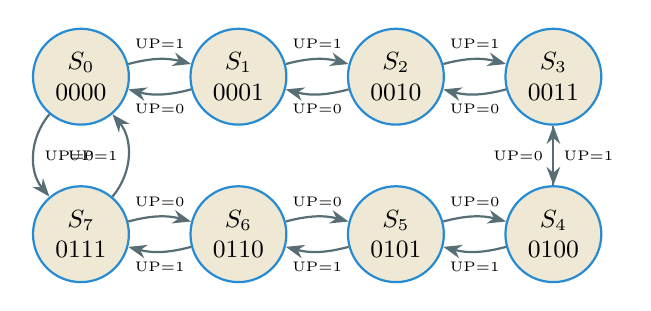
\begin{tikzpicture}[
    ->,>=Stealth,
    node distance=2cm,
    every state/.style={draw=solarizedBlue, fill=solarizedBase2, thick, minimum size=1cm, font=\small, align=center},
    every edge/.style={draw=solarizedBase01, thick}
]
    \node[state] (S0) {$S_0$\\0000};
    \node[state, right of=S0] (S1) {$S_1$\\0001};
    \node[state, right of=S1] (S2) {$S_2$\\0010};
    \node[state, right of=S2] (S3) {$S_3$\\0011};
    \node[state, below of=S3] (S4) {$S_4$\\0100};
    \node[state, left of=S4] (S5) {$S_5$\\0101};
    \node[state, left of=S5] (S6) {$S_6$\\0110};
    \node[state, left of=S6] (S7) {$S_7$\\0111};

    \path (S0) edge[bend left=15] node[above]{\tiny UP=1} (S1)
          (S1) edge[bend left=15] node[above]{\tiny UP=1} (S2)
          (S2) edge[bend left=15] node[above]{\tiny UP=1} (S3)
          (S3) edge node[right]{\tiny UP=1} (S4)
          (S4) edge[bend left=15] node[below]{\tiny UP=1} (S5)
          (S5) edge[bend left=15] node[below]{\tiny UP=1} (S6)
          (S6) edge[bend left=15] node[below]{\tiny UP=1} (S7)
          (S7) edge[bend right=40] node[left]{\tiny UP=1} (S0)

          (S1) edge[bend left=15] node[below]{\tiny UP=0} (S0)
          (S2) edge[bend left=15] node[below]{\tiny UP=0} (S1)
          (S3) edge[bend left=15] node[below]{\tiny UP=0} (S2)
          (S4) edge node[left]{\tiny UP=0} (S3)
          (S5) edge[bend left=15] node[above]{\tiny UP=0} (S4)
          (S6) edge[bend left=15] node[above]{\tiny UP=0} (S5)
          (S7) edge[bend left=15] node[above]{\tiny UP=0} (S6)
          (S0) edge[bend right=40] node[right]{\tiny UP=0} (S7);
\end{tikzpicture}
\end{center}
\begin{center}
    \textit{Figure 3: Up/Down Counter FSM (Moore Machine)}
\end{center}

\subsection{Design Approach}
This is a \textbf{Moore Machine} because:
\begin{itemize}
    \item The output (count) depends \textbf{only} on the current state
    \item Each state has a fixed output value regardless of input
    \item The UP\_DOWN input only affects the next state, not the output
\end{itemize}

\subsection{VHDL Implementation}
\macheader{up\_down\_counter.vhd}
\begin{lstlisting}[style=vhdlstyle]
library ieee;
use ieee.std_logic_1164.all;

entity up_down_counter is
    port (
        clk     : in std_logic;
        clr     : in std_logic;
        up_down : in std_logic;
        count   : out std_logic_vector (3 downto 0)
    );
end up_down_counter;

architecture bhv of up_down_counter is
    type state_type is (s0,s1,s2,s3,s4,s5,s6,s7);
    signal current_state, next_state : state_type;
begin

------------- Process 1: State Register -------------
    process (clk, clr)
    begin
        if clr = '1' then
            current_state <= s0;
        elsif rising_edge(clk) then
            current_state <= next_state;
        end if;
    end process;

------------- Process 2: Next State Logic -------------
    process (current_state, up_down)
    begin
        case current_state is
            when s0 =>
                if up_down = '1' then
                    next_state <= s1;
                else
                    next_state <= s7;
                end if;
            when s1 =>
                if up_down = '1' then
                    next_state <= s2;
                else
                    next_state <= s0;
                end if;
            when s2 =>
                if up_down = '1' then
                    next_state <= s3;
                else
                    next_state <= s1;
                end if;
            when s3 =>
                if up_down = '1' then
                    next_state <= s4;
                else
                    next_state <= s2;
                end if;
            when s4 =>
                if up_down = '1' then
                    next_state <= s5;
                else
                    next_state <= s3;
                end if;
            when s5 =>
                if up_down = '1' then
                    next_state <= s6;
                else
                    next_state <= s4;
                end if;
            when s6 =>
                if up_down = '1' then
                    next_state <= s7;
                else
                    next_state <= s5;
                end if;
            when s7 =>
                if up_down = '1' then
                    next_state <= s0;
                else
                    next_state <= s6;
                end if;
        end case;
    end process;

------------- Process 3: Output Logic (Moore) -------------
    process(current_state)
    begin
        case current_state is
            when s0 => count <= "0000";
            when s1 => count <= "0001";
            when s2 => count <= "0010";
            when s3 => count <= "0011";
            when s4 => count <= "0100";
            when s5 => count <= "0101";
            when s6 => count <= "0110";
            when s7 => count <= "0111";
        end case;
    end process;

end bhv;
\end{lstlisting}

\newpage
% ============== PRE-LAB PART 2 ==============
\section{Pre-Lab Part 2: "111" Sequence Detector (Mealy FSM)}

\subsection{FSM State Diagram}
\begin{center}
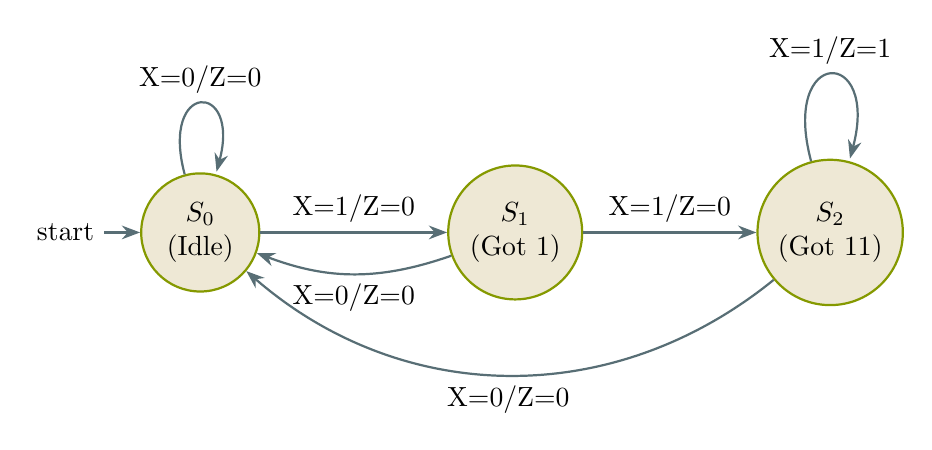
\begin{tikzpicture}[
    ->,>=Stealth,
    node distance=4cm,
    every state/.style={draw=solarizedGreen, fill=solarizedBase2, thick, minimum size=1.5cm, align=center},
    every edge/.style={draw=solarizedBase01, thick}
]
    \node[state, initial] (S0) {$S_0$\\(Idle)};
    \node[state, right of=S0] (S1) {$S_1$\\(Got 1)};
    \node[state, right of=S1] (S2) {$S_2$\\(Got 11)};

    \path (S0) edge[loop above] node{X=0/Z=0} (S0)
          (S0) edge node[above]{X=1/Z=0} (S1)
          (S1) edge[bend left=20] node[below]{X=0/Z=0} (S0)
          (S1) edge node[above]{X=1/Z=0} (S2)
          (S2) edge[bend left=40] node[below]{X=0/Z=0} (S0)
          (S2) edge[loop above] node{X=1/Z=1} (S2);
\end{tikzpicture}
\end{center}
\begin{center}
    \textit{Figure 4: "111" Sequence Detector - Mealy Machine}
\end{center}

\subsection{State Transition Table}
\begin{center}
\begin{tabular}{cccc}
\toprule
\textbf{Current State} & \textbf{Input X} & \textbf{Next State} & \textbf{Output Z} \\
\midrule
S0 (Idle) & 0 & S0 & 0 \\
S0 (Idle) & 1 & S1 & 0 \\
S1 (Got 1) & 0 & S0 & 0 \\
S1 (Got 1) & 1 & S2 & 0 \\
S2 (Got 11) & 0 & S0 & 0 \\
S2 (Got 11) & 1 & S2 & \textbf{1} \\
\bottomrule
\end{tabular}
\end{center}

\subsection{Why Mealy?}
\begin{itemize}
    \item Output Z=1 \textbf{immediately} when third '1' arrives (same clock cycle)
    \item Overlapping detection: stays in S2 after detection to catch consecutive "111" patterns
    \item Faster response than Moore (no extra state needed for output)
\end{itemize}

\subsection{VHDL Implementation}
\macheader{seq\_detector\_111\_mealy.vhd}
\begin{lstlisting}[style=vhdlstyle]
library ieee;
use ieee.std_logic_1164.all;

entity seq_detector_111_mealy is
    port (
        clk : in std_logic;
        rst : in std_logic;
        x   : in std_logic;
        z   : out std_logic
    );
end seq_detector_111_mealy;

architecture bhv of seq_detector_111_mealy is
    type state_type is (s0, s1, s2);
    signal current_state, next_state : state_type;
begin

------------- Process 1: State Register -------------
    process (clk, rst)
    begin
        if rst = '1' then
            current_state <= s0;
        elsif rising_edge(clk) then
            current_state <= next_state;
        end if;
    end process;

------------- Process 2: Next State Logic -------------
    process (current_state, x)
    begin
        case current_state is
            when s0 =>
                if x = '1' then
                    next_state <= s1;
                else
                    next_state <= s0;
                end if;
            when s1 =>
                if x = '1' then
                    next_state <= s2;
                else
                    next_state <= s0;
                end if;
            when s2 =>
                if x = '1' then
                    next_state <= s2;  -- Stay for overlapping
                else
                    next_state <= s0;
                end if;
        end case;
    end process;

------------- Process 3: Output Logic (Mealy) -------------
-- Output depends on BOTH current_state AND input x
    process (current_state, x)
    begin
        case current_state is
            when s0 => z <= '0';
            when s1 => z <= '0';
            when s2 =>
                if x = '1' then
                    z <= '1';  -- Immediate output!
                else
                    z <= '0';
                end if;
        end case;
    end process;

end bhv;
\end{lstlisting}

\newpage
% ============== IN-LAB TASK 1 ==============
\section{In-Lab Task 1: Even-Odd Up/Down Counter}

\subsection{FSM State Diagram}
The counter has two modes:
\begin{itemize}
    \item \textbf{Even Mode}: Cycles through 0, 2, 4, 6, 8, 10, 12, 14
    \item \textbf{Odd Mode}: Cycles through 1, 3, 5, 7, 9, 11, 13, 15
\end{itemize}

\begin{center}
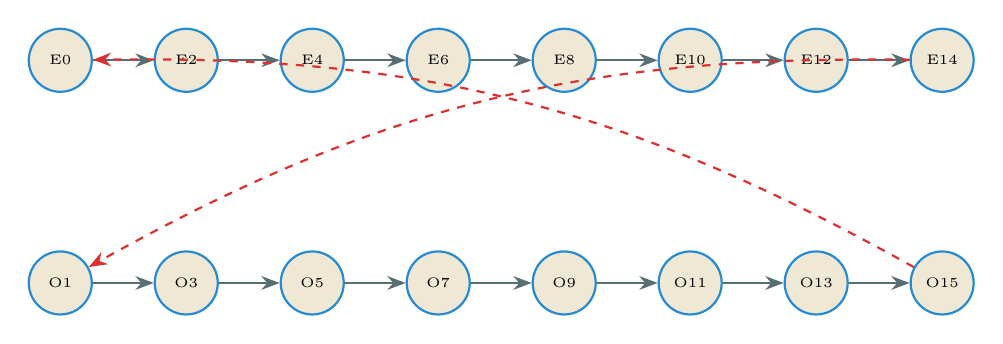
\begin{tikzpicture}[
    ->,>=Stealth,
    node distance=1.6cm,
    every state/.style={draw=solarizedBlue, fill=solarizedBase2, thick, minimum size=0.8cm, font=\tiny},
    every edge/.style={draw=solarizedBase01, thick, font=\tiny}
]
    % Even states (top row)
    \node[state] (E0) {E0};
    \node[state, right of=E0] (E2) {E2};
    \node[state, right of=E2] (E4) {E4};
    \node[state, right of=E4] (E6) {E6};
    \node[state, right of=E6] (E8) {E8};
    \node[state, right of=E8] (E10) {E10};
    \node[state, right of=E10] (E12) {E12};
    \node[state, right of=E12] (E14) {E14};

    % Odd states (bottom row)
    \node[state, below=2cm of E0] (O1) {O1};
    \node[state, right of=O1] (O3) {O3};
    \node[state, right of=O3] (O5) {O5};
    \node[state, right of=O5] (O7) {O7};
    \node[state, right of=O7] (O9) {O9};
    \node[state, right of=O9] (O11) {O11};
    \node[state, right of=O11] (O13) {O13};
    \node[state, right of=O13] (O15) {O15};

    % Even mode transitions (UP)
    \path (E0) edge node[above]{} (E2)
          (E2) edge node[above]{} (E4)
          (E4) edge node[above]{} (E6)
          (E6) edge node[above]{} (E8)
          (E8) edge node[above]{} (E10)
          (E10) edge node[above]{} (E12)
          (E12) edge node[above]{} (E14);

    % Switch from Even to Odd
    \path (E14) edge[bend right=15, dashed, color=solarizedRed] (O1);

    % Odd mode transitions (UP)
    \path (O1) edge node[below]{} (O3)
          (O3) edge node[below]{} (O5)
          (O5) edge node[below]{} (O7)
          (O7) edge node[below]{} (O9)
          (O9) edge node[below]{} (O11)
          (O11) edge node[below]{} (O13)
          (O13) edge node[below]{} (O15);

    % Switch from Odd to Even
    \path (O15) edge[bend right=15, dashed, color=solarizedRed] (E0);
\end{tikzpicture}
\end{center}
\begin{center}
    \textit{Figure 5: Even-Odd Counter FSM (Moore Machine) - UP direction shown}
\end{center}

\textbf{Note:} DOWN direction reverses all transitions. Dashed red arrows show mode switching.

\subsection{VHDL Implementation}
\macheader{even\_odd\_counter.vhd}
\begin{lstlisting}[style=vhdlstyle]
library ieee;
use ieee.std_logic_1164.all;

entity even_odd_counter is
    port (
        clk   : in std_logic;
        rst   : in std_logic;
        cen   : in std_logic;  -- Counter enable
        dir   : in std_logic;  -- Direction: 1=UP, 0=DOWN
        count : out std_logic_vector(3 downto 0)
    );
end even_odd_counter;

architecture bhv of even_odd_counter is
    type state_type is (e0, e2, e4, e6, e8, e10, e12, e14,
                        o1, o3, o5, o7, o9, o11, o13, o15);
    signal current_state, next_state : state_type;
begin

------------- Process 1: State Register -------------
    process (clk, rst)
    begin
        if rst = '1' then
            current_state <= e0;
        elsif rising_edge(clk) then
            if cen = '1' then
                current_state <= next_state;
            end if;
        end if;
    end process;

------------- Process 2: Next State Logic -------------
    process (current_state, dir)
    begin
        case current_state is
            -- Even Mode States
            when e0 =>
                if dir = '1' then next_state <= e2;
                else next_state <= o15;
                end if;
            when e2 =>
                if dir = '1' then next_state <= e4;
                else next_state <= e0;
                end if;
            when e4 =>
                if dir = '1' then next_state <= e6;
                else next_state <= e2;
                end if;
            when e6 =>
                if dir = '1' then next_state <= e8;
                else next_state <= e4;
                end if;
            when e8 =>
                if dir = '1' then next_state <= e10;
                else next_state <= e6;
                end if;
            when e10 =>
                if dir = '1' then next_state <= e12;
                else next_state <= e8;
                end if;
            when e12 =>
                if dir = '1' then next_state <= e14;
                else next_state <= e10;
                end if;
            when e14 =>
                if dir = '1' then next_state <= o1;
                else next_state <= e12;
                end if;
            -- Odd Mode States
            when o1 =>
                if dir = '1' then next_state <= o3;
                else next_state <= e14;
                end if;
            when o3 =>
                if dir = '1' then next_state <= o5;
                else next_state <= o1;
                end if;
            when o5 =>
                if dir = '1' then next_state <= o7;
                else next_state <= o3;
                end if;
            when o7 =>
                if dir = '1' then next_state <= o9;
                else next_state <= o5;
                end if;
            when o9 =>
                if dir = '1' then next_state <= o11;
                else next_state <= o7;
                end if;
            when o11 =>
                if dir = '1' then next_state <= o13;
                else next_state <= o9;
                end if;
            when o13 =>
                if dir = '1' then next_state <= o15;
                else next_state <= o11;
                end if;
            when o15 =>
                if dir = '1' then next_state <= e0;
                else next_state <= o13;
                end if;
        end case;
    end process;

------------- Process 3: Output Logic (Moore) -------------
    process (current_state)
    begin
        case current_state is
            when e0  => count <= "0000";
            when e2  => count <= "0010";
            when e4  => count <= "0100";
            when e6  => count <= "0110";
            when e8  => count <= "1000";
            when e10 => count <= "1010";
            when e12 => count <= "1100";
            when e14 => count <= "1110";
            when o1  => count <= "0001";
            when o3  => count <= "0011";
            when o5  => count <= "0101";
            when o7  => count <= "0111";
            when o9  => count <= "1001";
            when o11 => count <= "1011";
            when o13 => count <= "1101";
            when o15 => count <= "1111";
        end case;
    end process;

end bhv;
\end{lstlisting}

\newpage
% ============== IN-LAB TASK 2 ==============
\section{In-Lab Task 2: "1101" Sequence Detector}

\subsection{Understanding the Problem}
We need to detect the sequence \textbf{"1101"} in a serial bit stream. Key questions:
\begin{itemize}
    \item What happens when we receive each bit?
    \item How do we handle \textbf{overlapping patterns}? (e.g., "110\textbf{1101}" has two "1101" patterns sharing bits)
\end{itemize}

\subsection{Step-by-Step FSM Construction}

\textbf{Pattern to detect:} 1 $\rightarrow$ 1 $\rightarrow$ 0 $\rightarrow$ 1

\begin{center}
\begin{tabular}{|c|l|l|}
\hline
\textbf{State} & \textbf{What we've matched so far} & \textbf{Waiting for} \\
\hline
S0 & Nothing (or mismatch occurred) & First '1' \\
S1 & "1" & Second '1' \\
S2 & "11" & '0' \\
S3 & "110" & Final '1' \\
S4 & "1101" - COMPLETE! & (Output Z=1) \\
\hline
\end{tabular}
\end{center}

\subsection{Tricky Transitions Explained}

\textbf{1. Why does S2 loop on input '1'?}
\begin{itemize}
    \item In S2, we have "11". If we get another '1', we now have "111"
    \item The last two bits "11" are still a valid partial match for "1101"
    \item So we stay in S2 (we still have "11" matched)
\end{itemize}

\textbf{2. Why does S4 go to S2 on input '1'?}
\begin{itemize}
    \item In S4, we just detected "1101". If next input is '1':
    \item The sequence "1101\textbf{1}" ends with "1" which could start a new "1101"
    \item Actually, "01" at the end + new "1" = we have "1" matched $\rightarrow$ but wait!
    \item "1101" ends with "01", and if we get "1", we have "011" - only last "1" useful
    \item But "1101" also contains "1" at position 4, so go to S1? No!
    \item Actually: "1101" + "1" = "11011". Looking backward: "11" is matched $\rightarrow$ S2
\end{itemize}

\textbf{3. Why does S3 go to S0 on input '0'?}
\begin{itemize}
    \item In S3, we have "110". If we get '0', we have "1100"
    \item No suffix of "1100" matches any prefix of "1101"
    \item Start over from S0
\end{itemize}

%------ MOORE FSM DIAGRAM ------
\subsection{Moore Machine: FSM State Diagram}
\begin{center}
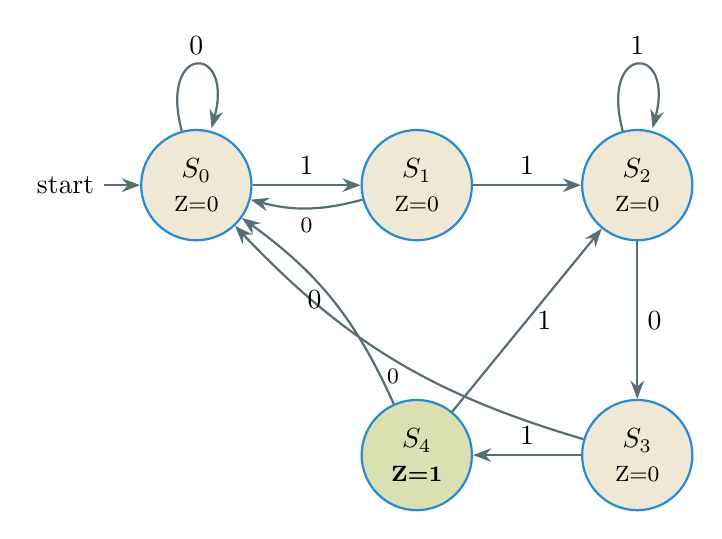
\begin{tikzpicture}[
    ->,>=Stealth,
    node distance=2.8cm,
    every state/.style={draw=solarizedBlue, fill=solarizedBase2, thick, minimum size=1.4cm, align=center},
    every edge/.style={draw=solarizedBase01, thick}
]
    \node[state, initial] (S0) {$S_0$\\{\footnotesize Z=0}};
    \node[state, right of=S0] (S1) {$S_1$\\{\footnotesize Z=0}};
    \node[state, right of=S1] (S2) {$S_2$\\{\footnotesize Z=0}};
    \node[state, below=2cm of S2] (S3) {$S_3$\\{\footnotesize Z=0}};
    \node[state, left of=S3, fill=solarizedGreen!30] (S4) {$S_4$\\{\footnotesize \textbf{Z=1}}};

    % Transitions with clear labels
    \path (S0) edge[loop above] node{0} (S0)
          (S0) edge node[above]{1} (S1)
          (S1) edge[bend left=15] node[below]{\footnotesize 0} (S0)
          (S1) edge node[above]{1} (S2)
          (S2) edge node[right]{0} (S3)
          (S2) edge[loop above] node{1} (S2)
          (S3) edge[bend left=15] node[below]{\footnotesize 0} (S0)
          (S3) edge node[above]{1} (S4)
          (S4) edge[bend right=15] node[left]{0} (S0)
          (S4) edge node[right]{1} (S2);
\end{tikzpicture}
\end{center}
\begin{center}
    \textit{Figure 6: "1101" Sequence Detector - Moore Machine (Output in state)}
\end{center}

\subsection{Moore: Complete State Transition Table}
\begin{center}
\begin{tabular}{|c|c|c|c|c|}
\hline
\textbf{Current} & \textbf{Matched} & \textbf{Input} & \textbf{Next} & \textbf{Output Z} \\
\textbf{State} & \textbf{Pattern} & \textbf{X} & \textbf{State} & \textbf{(Moore)} \\
\hline
S0 & --- & 0 & S0 & 0 \\
S0 & --- & 1 & S1 & 0 \\
\hline
S1 & "1" & 0 & S0 & 0 \\
S1 & "1" & 1 & S2 & 0 \\
\hline
S2 & "11" & 0 & S3 & 0 \\
S2 & "11" & 1 & S2 & 0 \\
\hline
S3 & "110" & 0 & S0 & 0 \\
S3 & "110" & 1 & S4 & 0 \\
\hline
S4 & "1101" & 0 & S0 & \textbf{1} \\
S4 & "1101" & 1 & S2 & \textbf{1} \\
\hline
\end{tabular}
\end{center}

\subsection{Moore VHDL Implementation}
\macheader{seq\_detector\_1101\_moore.vhd}
\begin{lstlisting}[style=vhdlstyle]
library ieee;
use ieee.std_logic_1164.all;

entity seq_detector_1101_moore is
    port (
        clk : in std_logic;
        rst : in std_logic;
        x   : in std_logic;
        z   : out std_logic
    );
end seq_detector_1101_moore;

architecture bhv of seq_detector_1101_moore is
    -- S0: nothing matched
    -- S1: matched "1"
    -- S2: matched "11"
    -- S3: matched "110"
    -- S4: matched "1101" -> OUTPUT!
    type state_type is (s0, s1, s2, s3, s4);
    signal current_state, next_state : state_type;
begin

------------- Process 1: State Register -------------
    process (clk, rst)
    begin
        if rst = '1' then
            current_state <= s0;
        elsif rising_edge(clk) then
            current_state <= next_state;
        end if;
    end process;

------------- Process 2: Next State Logic -------------
    process (current_state, x)
    begin
        case current_state is
            when s0 =>  -- Nothing matched yet
                if x = '1' then
                    next_state <= s1;  -- Got first '1'
                else
                    next_state <= s0;  -- Stay, wait for '1'
                end if;

            when s1 =>  -- Matched "1"
                if x = '1' then
                    next_state <= s2;  -- Got "11"
                else
                    next_state <= s0;  -- "10" - no match, restart
                end if;

            when s2 =>  -- Matched "11"
                if x = '1' then
                    next_state <= s2;  -- "111" -> still have "11"
                else
                    next_state <= s3;  -- Got "110"
                end if;

            when s3 =>  -- Matched "110"
                if x = '1' then
                    next_state <= s4;  -- Got "1101" - DETECTED!
                else
                    next_state <= s0;  -- "1100" - no useful suffix
                end if;

            when s4 =>  -- Matched "1101" - OUTPUT STATE
                if x = '1' then
                    next_state <= s2;  -- "11011" ends with "11"
                else
                    next_state <= s0;  -- "11010" - restart
                end if;
        end case;
    end process;

------------- Process 3: Output Logic (Moore) -------------
-- Moore: Output depends ONLY on current state
    process (current_state)
    begin
        case current_state is
            when s0 => z <= '0';
            when s1 => z <= '0';
            when s2 => z <= '0';
            when s3 => z <= '0';
            when s4 => z <= '1';  -- OUTPUT HERE!
        end case;
    end process;

end bhv;
\end{lstlisting}

\newpage
%------ MEALY FSM ------
\subsection{Mealy Machine: FSM State Diagram}

In Mealy, output appears on the \textbf{transition} (immediately when final '1' arrives), not after entering a state. This means we need \textbf{only 4 states} (no S4 needed).

\begin{center}
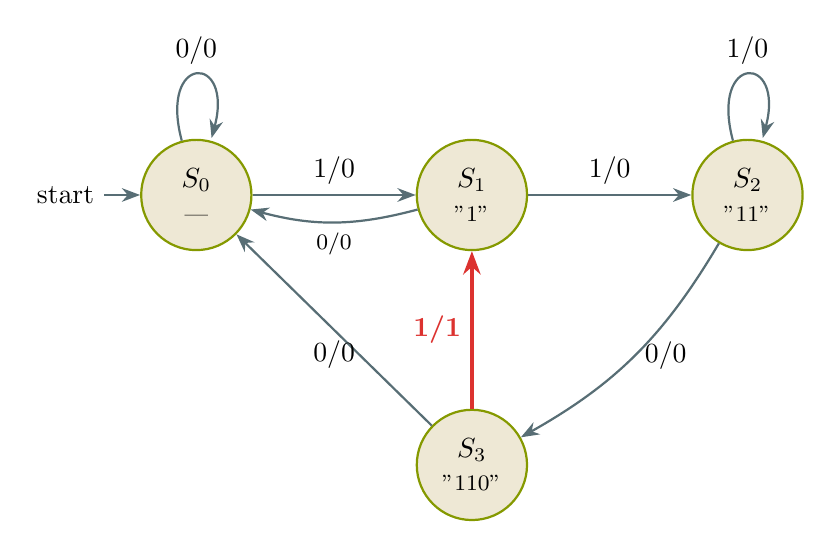
\begin{tikzpicture}[
    ->,>=Stealth,
    node distance=3.5cm,
    every state/.style={draw=solarizedGreen, fill=solarizedBase2, thick, minimum size=1.4cm, align=center},
    every edge/.style={draw=solarizedBase01, thick}
]
    \node[state, initial] (S0) {$S_0$\\{\footnotesize ---}};
    \node[state, right of=S0] (S1) {$S_1$\\{\footnotesize "1"}};
    \node[state, right of=S1] (S2) {$S_2$\\{\footnotesize "11"}};
    \node[state, below=2cm of S1] (S3) {$S_3$\\{\footnotesize "110"}};

    % Transitions with input/output labels
    \path (S0) edge[loop above] node{0/0} (S0)
          (S0) edge node[above]{1/0} (S1)
          (S1) edge[bend left=15] node[below]{\footnotesize 0/0} (S0)
          (S1) edge node[above]{1/0} (S2)
          (S2) edge[bend left=15] node[right]{0/0} (S3)
          (S2) edge[loop above] node{1/0} (S2)
          (S3) edge node[below]{0/0} (S0)
          (S3) edge[color=solarizedRed, very thick] node[left]{\textbf{1/1}} (S1);
\end{tikzpicture}
\end{center}
\begin{center}
    \textit{Figure 7: "1101" Sequence Detector - Mealy Machine (Output on transition)}
\end{center}

\textbf{Key Difference:} The red arrow shows Z=1 output \textbf{immediately} when the final '1' arrives, while transitioning to S1 (since "1101" ends with "1").

\subsection{Mealy: Complete State Transition Table}
\begin{center}
\begin{tabular}{|c|c|c|c|c|}
\hline
\textbf{Current} & \textbf{Matched} & \textbf{Input} & \textbf{Next} & \textbf{Output Z} \\
\textbf{State} & \textbf{Pattern} & \textbf{X} & \textbf{State} & \textbf{(Mealy)} \\
\hline
S0 & --- & 0 & S0 & 0 \\
S0 & --- & 1 & S1 & 0 \\
\hline
S1 & "1" & 0 & S0 & 0 \\
S1 & "1" & 1 & S2 & 0 \\
\hline
S2 & "11" & 0 & S3 & 0 \\
S2 & "11" & 1 & S2 & 0 \\
\hline
S3 & "110" & 0 & S0 & 0 \\
S3 & "110" & 1 & S1 & \textbf{1} $\leftarrow$ Immediate! \\
\hline
\end{tabular}
\end{center}

\subsection{Mealy VHDL Implementation}
\macheader{seq\_detector\_1101\_mealy.vhd}
\begin{lstlisting}[style=vhdlstyle]
library ieee;
use ieee.std_logic_1164.all;

entity seq_detector_1101_mealy is
    port (
        clk : in std_logic;
        rst : in std_logic;
        x   : in std_logic;
        z   : out std_logic
    );
end seq_detector_1101_mealy;

architecture bhv of seq_detector_1101_mealy is
    -- Only 4 states needed (no output state)
    -- S0: nothing matched
    -- S1: matched "1"
    -- S2: matched "11"
    -- S3: matched "110"
    type state_type is (s0, s1, s2, s3);
    signal current_state, next_state : state_type;
begin

------------- Process 1: State Register -------------
    process (clk, rst)
    begin
        if rst = '1' then
            current_state <= s0;
        elsif rising_edge(clk) then
            current_state <= next_state;
        end if;
    end process;

------------- Process 2: Next State Logic -------------
    process (current_state, x)
    begin
        case current_state is
            when s0 =>
                if x = '1' then
                    next_state <= s1;
                else
                    next_state <= s0;
                end if;

            when s1 =>
                if x = '1' then
                    next_state <= s2;
                else
                    next_state <= s0;
                end if;

            when s2 =>
                if x = '1' then
                    next_state <= s2;  -- "111" -> "11"
                else
                    next_state <= s3;  -- "110"
                end if;

            when s3 =>
                if x = '1' then
                    next_state <= s1;  -- "1101" -> "1" (output here!)
                else
                    next_state <= s0;
                end if;
        end case;
    end process;

------------- Process 3: Output Logic (Mealy) -------------
-- Mealy: Output depends on state AND input
    process (current_state, x)
    begin
        z <= '0';  -- Default output
        case current_state is
            when s0 => z <= '0';
            when s1 => z <= '0';
            when s2 => z <= '0';
            when s3 =>
                if x = '1' then
                    z <= '1';  -- IMMEDIATE OUTPUT!
                else
                    z <= '0';
                end if;
        end case;
    end process;

end bhv;
\end{lstlisting}

\newpage
% ============== TIMING COMPARISON ==============
\section{Timing Comparison: Moore vs Mealy}

\subsection{Example Input: "1101101"}

\textbf{Moore Machine Timing:}
\begin{center}
\begin{tabular}{|c|c|c|c|c|c|c|c|c|}
\hline
\textbf{Clock} & 0 & 1 & 2 & 3 & 4 & 5 & 6 & 7 \\
\hline
\textbf{Input X} & - & 1 & 1 & 0 & 1 & 1 & 0 & 1 \\
\hline
\textbf{State} & S0 & S1 & S2 & S3 & \cellcolor{solarizedGreen!30}S4 & S2 & S3 & \cellcolor{solarizedGreen!30}S4 \\
\hline
\textbf{Output Z} & 0 & 0 & 0 & 0 & \textbf{1} & 0 & 0 & \textbf{1} \\
\hline
\end{tabular}
\end{center}

\textbf{Mealy Machine Timing:}
\begin{center}
\begin{tabular}{|c|c|c|c|c|c|c|c|c|}
\hline
\textbf{Clock} & 0 & 1 & 2 & 3 & 4 & 5 & 6 & 7 \\
\hline
\textbf{Input X} & - & 1 & 1 & 0 & 1 & 1 & 0 & 1 \\
\hline
\textbf{State} & S0 & S1 & S2 & S3 & S1 & S2 & S3 & S1 \\
\hline
\textbf{Output Z} & 0 & 0 & 0 & 0 & \textbf{1}$^*$ & 0 & 0 & \textbf{1}$^*$ \\
\hline
\end{tabular}
\end{center}
$^*$Output appears \textbf{during} clock cycle 4, not after.

\subsection{Key Observations}
\begin{enumerate}
    \item \textbf{Moore}: Output appears in clock cycle 4 (after entering S4)
    \item \textbf{Mealy}: Output appears during the transition in cycle 4 (immediately with input)
    \item \textbf{Moore needs 5 states}, Mealy needs only 4 states
    \item \textbf{Moore output is more stable} (synchronized with clock)
    \item \textbf{Mealy responds faster} (no extra clock delay)
\end{enumerate}

% ============== CONCLUSION ==============
\section{Conclusion}

This lab demonstrated:
\begin{enumerate}
    \item \textbf{Moore Machines}: Used for counters and sequence detectors where output stability is important (output changes only on clock edges)
    \item \textbf{Mealy Machines}: Used when immediate response is needed (output changes asynchronously with input)
    \item \textbf{FSM Design Pattern}: Three-process architecture (state register, next-state logic, output logic) provides clean separation of concerns
    \item \textbf{Overlapping Detection}: Critical for sequence detectors - the FSM must transition to an appropriate state to catch consecutive patterns
\end{enumerate}

\end{document}
